\documentclass[a4paper,10pt]{cas-dc} % double-column style

% Elsevier/ECM manuscript source converted from Word draft.
% Temporary citation placeholders are written as [Cite X].
% Replace them with \cite{...} commands and add your .bib file when the bibliography is ready.

\usepackage[utf8]{inputenc}
\usepackage[T1]{fontenc}
\usepackage{textcomp}
\usepackage{amsmath,amssymb}
\usepackage{graphicx}
\usepackage{booktabs}
\usepackage{longtable}
\usepackage{array}
\usepackage{calc}
\usepackage{float}
\usepackage{placeins}
\usepackage{subcaption}
\usepackage{url}
\hypersetup{
    colorlinks=true,
    linkcolor=blue,
    citecolor=red,
    urlcolor=brown,    
    filecolor=blue
}

\usepackage{lineno}
\usepackage{setspace}

% Relax float placement rules so figures/tables stay close to their citations
\renewcommand{\topfraction}{0.95}
\renewcommand{\bottomfraction}{0.8}
\renewcommand{\textfraction}{0.05}
\renewcommand{\floatpagefraction}{0.7}
\renewcommand{\dbltopfraction}{0.95}
\renewcommand{\dblfloatpagefraction}{0.7}
\setcounter{topnumber}{3}
\setcounter{totalnumber}{4}
\setcounter{dbltopnumber}{3}

\begin{document}

\shorttitle{}
\shortauthors{J. Park et~al.}

\title{Parametric Investigation of the Operating Limits and Performance Effects of Anode Off-Gas Recirculation in Ammonia-Fueled Solid Oxide Fuel Cell Systems}

\author[yonsei]{Jaeyoung Park}
\author[yonsei]{Kwangnam Jeong}
\author[yonsei]{Taewook Lee}
\author[yonsei]{Jongsup Hong}
\cormark[1]
\ead{jongsup.hong@yonsei.ac.kr}
\cortext[cor1]{Corresponding author.}

\affiliation[yonsei]{organization={School of Mechanical Engineering, Yonsei University},
            addressline={50 Yonsei-ro, Seodaemun-gu},
            city={Seoul},
            postcode={03722},
            country={South Korea}}

\begin{abstract}
Ammonia-fueled solid oxide fuel cell (SOFC) systems with anode off-gas recirculation (AOGR) offer high efficiency for marine power generation, but their performance is strongly coupled to operating conditions and the AOGR ratio.
However, previous studies have generally treated AOGR ratio as a freely adjustable design input rather than a physically constrained outcome, and have examined its effect along a single operating axis.
This study addresses these limitations by identifying the physically attainable maximum AOGR ratio and quantifying its interaction with operating conditions through a two-dimensional parametric study spanning fuel utilization, current density, and stack inlet temperature. 
The analysis was conducted using an integrated thermodynamic system model incorporating validated component models, implemented within an in-house thermodynamic simulator.
Results show that increasing fuel utilization from 40\% to 80\% raises the maximum AOGR ratio from 65.4\% to 66.9\%, whereas increasing current density from 0.1 to 0.5 A/cm² lowers it from 67.3\% to 62.0\%. 
Elevated stack inlet temperature further restricts this limit by degrading ejector entrainment performance. 
The AOGR ratio consistently improves efficiency while reducing power density, with the largest efficiency gains occurring at low fuel utilization. 
In addition, the optimal stack operating temperature shifts downward as the AOGR ratio increases. 
At high current density, growing balance-of-plant parasitic power produces a non-monotonic efficiency trend, yielding an optimal AOGR ratio below its maximum allowable value. 
These findings demonstrate that the AOGR ratio, operating conditions, and system constraints must be co-optimized for effective ammonia-fueled SOFC system design.
\end{abstract}

\begin{keywords}
Solid oxide fuel cell \sep Marine power source \sep Ammonia \sep Anode off-gas recirculation \sep Ejector \sep Parametric study
\end{keywords}

\maketitle

% \linenumbers    % re-enable for review submission
\doublespacing
\setdisplayskipstretch{1.0}% keep normal spacing around display equations despite double spacing

\section{Introduction}

The maritime industry is currently undergoing a major transition toward decarbonization, driven by tightening international regulations on greenhouse gas emissions and the long-term goal of achieving net-zero shipping \cite{ROBALOCABRERA2025104549,IMO2023GHGStrategy}.
As conventional marine fuels such as heavy fuel oil and marine diesel oil are no longer compatible with these targets, the search for clean and energy-dense alternative fuels has become a central topic in marine power generation research \cite{ALENAZI20211962}.
Among the candidates proposed thus far, ammonia has emerged as one of the most prominent options because it contains no carbon and can therefore be utilized without any direct CO$_2$ emission \cite{su152115565}.
Compared with hydrogen, which has often been regarded as the ultimate clean fuel but suffers from cryogenic storage requirements and low volumetric energy density, ammonia can be stored and transported as a pressurized liquid under significantly milder conditions, making it far more practical for shipboard storage where space and weight constraints are critical \cite{en13123062,MCKINLAY202128282}.
Furthermore, an extensive global infrastructure for ammonia production, transportation, and bunkering has already been established for fertilizer use, providing a uniquely favorable starting point for its near-term deployment as a marine fuel \cite{Ammonfuel2020}.

To convert ammonia fuel into electrical power onboard, a power conversion device that combines high efficiency with operational compatibility with ammonia is required.
Internal combustion engines are an option currently under active development, but their combustion processes inherently produce NOx and N$_2$O emissions that necessitate additional flue-gas treatment systems \cite{Nygard2025N2ORemoval}.
Fuel cells, in contrast, electrochemically convert fuel into electricity without combustion, thereby offering both higher efficiency and substantially cleaner emissions \cite{VANBIERT2016345}.
Among various fuel cell types investigated for ammonia operation, solid oxide fuel cell (SOFC) is particularly well-suited because its high operating temperature, typically between 600 and 900 \textdegree C, simultaneously provides high thermodynamic efficiency and the thermal driving force necessary to decompose ammonia into hydrogen and nitrogen \cite{10.1039/d3qi01557b,10.1039/d0ta08810b}.
For these reasons, ammonia-fueled SOFCs have rapidly emerged as a strong candidate for next-generation marine power generation systems pursuing zero-emission shipping.

Reflecting such potential, extensive research efforts have been conducted on ammonia-fueled SOFC systems, ranging from fundamental electrochemical performance evaluation to system-level thermodynamic analysis \cite{WOJCIK2003342,CINTI201613583,ISHAK2012157,LEE2025238271,ISHAK201273}.
Wojcik et al.~\cite{WOJCIK2003342} experimentally evaluated ammonia as a fuel for SOFCs and demonstrated that ammonia-fed operation can achieve performance comparable to hydrogen-fed operation when ammonia decomposition is effectively promoted over suitable catalyst materials.
Cinti et al.~\cite{CINTI201613583} combined ammonia-fed SOFC stack testing with system-level analysis and showed that SOFC operation with ammonia is technically feasible.
Ishak et al.~\cite{ISHAK2012157} performed thermodynamic analysis of ammonia-fed SOFCs and showed that ammonia can serve as an effective hydrogen carrier for SOFC operation, with system performance strongly affected by operating conditions such as stack temperature and fuel utilization.
Lee et al.~\cite{LEE2025238271} thermodynamically compared internal and external ammonia decomposition strategies for ammonia-fueled SOFC systems, showing that thermal integration methods and system configurations can greatly affect system performance.
Ishak et al.~\cite{ISHAK201273} conducted energy and exergy analyses of direct ammonia SOFC system integrated with a gas turbine cycle, showing that the hybrid configuration can effectively utilize SOFC waste heat for combined heat and power generation, improving overall system performance.

Previous studies have demonstrated that the performance of SOFC systems is strongly influenced by a wide range of design and operating parameters.
A promising design strategy to enhance the electrical efficiency of SOFC systems is anode off-gas recirculation (AOGR).
AOGR improves system electrical efficiency by decreasing the amount of fresh fuel consumption at a fixed SOFC stack fuel utilization condition, thereby increasing the net system fuel utilization \cite{TORII2016229}.
To thoroughly analyze the effect of AOGR on ammonia-fueled SOFC systems, various studies have been conducted.
Selvam et al.~\cite{SELVAM2021114839} thermodynamically analyzed a full AOGR ammonia-fueled SOFC system achieving 100\% system fuel utilization, showing that the full AOGR strategy improves energy and exergy efficiencies by 12.17 and 11.39 percentage points, respectively, over a conventional system.
Jeong et al, Bąkała et al.~\cite{JEONG2026101799,BAKALA2024952} compared the performance of SOFC systems fueled with hydrogen, natural gas and ammonia, under both with and without AOGR.
Both studies revealed that AOGR generally tends to improve system electrical efficiency, regardless of fuel types.
Quach et al.~\cite{QUACH2022119718} studied the effect of water removal at the anode off-gas via condensation in ammonia-fueled SOFC system, and further improved system performance via integration of an internal combustion engine.
The efficiency of AOGR system with water removal was 12.7 percentage point higher than that of a standalone system, and was only 0.1 percentage point lower than that of a AOGR system utilizing both water removal and internal combustion engine.
Sun et al.~\cite{SUN2023117804} conducted a parametric study to analyze how operating conditions such as current density, AOGR ratio, etc. affects the system performance of an ammonia-fueled SOFC system.
Oh et al.~\cite{OH2024235241}  also conducted a parametric study to find the optimal operating condition of an ammonia fueled-SOFC system undergoing AOGR, integrated with an organic Rankine cycle.

However, while previous studies focus on proposing high-efficiency system architectures, they tend to lack practical thermodynamic considerations in system evaluation regarding AOGR.
First, prior studies consider AOGR ratio as an independently adjustable operating variable, whereas in practice an upper bound may exist due to physical constraints \cite{SELVAM2021114839, QUACH2022119718, SUN2023117804, OH2024235241}.
Second, the influence of AOGR ratio has typically been examined along a single operating axis at a fixed fuel utilization or current density, leaving the coupling between AOGR ratio and other operating variables unexplored \cite{QUACH2022119718, SUN2023117804, OH2024235241}.
Third, prior studies either do not account for or assume a designated value for pressure drop effects at heat exchangers \cite{SELVAM2021114839, BAKALA2024952, QUACH2022119718, SUN2023117804, OH2024235241}.
Furthermore, in systems utilizing an ejector for AOGR, the ejector model is overly simplified as a component which mixes two streams and pressurizes the entrained flow by a fixed pressure ratio \cite{SUN2023117804}.

To address such limitations, the present study pursues the following research objectives with the following novelties:

\begin{itemize}
\item The physically attainable maximum AOGR ratio is identified as an endogenous outcome of component level hydrodynamics under varying stack inlet temperature, fuel utilization, and current density, rather than being prescribed as an external design input.
\item A two-dimensional parametric study is conducted in a system level to reveal how the AOGR ratio couples with each operating variables, thereby analyzing the mechanisms by which the AOGR ratio influences overall system performance under realistic operating conditions.
\item A high-fidelity ammonia-fueled SOFC system model is developed using an in-house simulator, in which pressure drops across balance of plant components are evaluated through empirical correlation based physical models accounting for design variables, and the AOGR is described by a reliable one-dimensional ejector model that captures the entrainment-pressure-lift behavior.
\end{itemize}

\section{Thermodynamic Component Modeling Methodology}

To study the performance of ammonia -- fueled SOFC systems under various operating conditions, thermodynamic systems were computationally modelled and analyzed via numerical simulation.
Numerical simulations were conducted via an in-house solid oxide cell system simulator developed in C\# language, H-Twin\textsuperscript{\textregistered} (H-Cube Solutions).
The thermodynamic systems consisted of system components, fluid streams, and an integrated system.
An integrated system was assembled by a set of system components which are connected by fluid streams represented by thermodynamic properties including mass flow rate (\(\dot{m})\), temperature \((T)\), pressure \((p)\) and chemical composition \((x)\).
The system components of an ammonia -- fueled SOFC system include SOFC stack, heat exchanger, ammonia cracker, combustor, blower, etc.
In addition, if the system undergoes AOGR, an ejector is also included to induce suction of the relatively low-pressure anode off -- gas.
Thermodynamic properties are calculated for each stream via a steady -- state numerical solver, where each system component calculates the thermodynamic properties of its outlet stream as the output, given the inlet stream and its design configurations as the input.
Numerical values of thermodynamic properties were acquired from the following sources: thermodynamic properties of water~\cite{Wagner2008}, specific heat capacities of gases~\cite{Smith1999GRIMech30}, thermal conductivity and dynamic viscosity of gases~\cite{TODD2002186}, and enthalpy of formation of gases~\cite{moran2017moran}.
Design configuration of system components include geometrical design variables and operational parameters.
For example, in the case of SOFC stack, geometrical design variables such as cell dimensions, fluid channel dimensions and operational parameters such as current density are determined as design configurations.
Together with the design configurations and thermodynamic properties of its cathode/anode inlet stream as the input, the thermodynamic properties of its outlet streams and voltage, power generation values are calculated as the output by solving internal electrochemistry and mass/energy balance equations.
Throughout the study, key assumptions applied are as follows:

\begin{itemize}
\item For chemical species, only H$_2$, H$_2$O, CO, CO$_2$, O$_2$, N$_2$, CH$_4$, NH$_3$ are considered.
\item For the equation of state, only H$_2$O is modeled as a real gas while other gases are modeled as ideal gases.
\item In energy conservation, kinetic and potential energy are neglected.
\item All system components assume an adiabatic condition between the component and the environment.
\item Radiative heat transfer is neglected.
\item Steady-state operation is assumed.
\item Pressure drop does not occur in pipes when connecting components.
\item Effect of stacking SOFC cells is neglected.
\end{itemize}

\subsection{SOFC Stack}

A 1 -- dimensional model of SOFC stack developed by Min et al.~\cite{MIN2020112614} was exploited to calculate the voltage, power generation and thermodynamic properties of its outlet streams.
The model considers discretized sections of a SOFC stack in the direction of fuel flow and solves complete analytical expressions of electrochemical, thermodynamic relations for each section to derive its output parameters.
Given the input parameters, internal electrochemical reaction is solved and the local value of voltage of each section is calculated by the following equations.

\begin{align}
V &= E_{eq} - \eta_{act,a} - \eta_{act,c} - \eta_{ohm} - \eta_{conc,a} - \eta_{conc,c} \label{eq:cell-voltage} \\
E_{eq} &= \  - \frac{\mathrm{\Delta}G{^\circ}}{2F} + \frac{RT}{2F}\ln\left( \frac{p_{H_{2}}{p_{O_{2}}}^{\frac{1}{2}}}{p_{H_{2}O}} \right) \label{eq:nernst}
\end{align}

Detailed equations and parameters of overpotentials are provided in \cite{MIN2020112614}.
The calculated values of voltage at each section are averaged to derive the final voltage of the stack.
Based on the value of voltage, design configurations and operational parameters of the stack, gross power generation is calculated by the following equation.

\begin{equation}
{\dot{W}}_{gross} = jA_{cell}N_{cell}V_{SOFC} \label{eq:gross-power}
\end{equation}

Along with the calculation of voltage, the heat generated from electrochemical reaction is utilized for outlet gases post -- heating, satisfying the mass, energy and heat balance in each section and the overall stack.
Simulation results of the model has been validated with experimental results for hydrogen operation.
Since this study considers ammonia to be decomposed in a reformer before entering the SOFC anode channel -- where the equilibrium assumption of temperature over 600\textdegree C yields a conversion rate exceeding 99.9\% - the anode channel gas can be treated as diluted hydrogen \cite{fuerte2009ammonia,lucentini2019catalytic, maffei2008high}.
Therefore, it can be considered that the model provides reliable results for ammonia operations.

\subsection{Balance of Plants (BoPs)}

\subsubsection{Heat Exchanger}

A shell and tube heat exchanger model developed by Park et al.~\cite{park2019comparative} was employed to transfer heat from post -- combustion gas to fresh air.
Fresh air flows into the tube side of the heat exchanger as the cold fluid, and post combustion gas enters the shell side as the hot fluid.
The model takes geometrical parameters such as tube length, shell diameter, number of baffles, etc. and thermodynamic properties of inlet gases as the input to calculate output values such as pressure drops, heat transfer coefficient, outlet gas temperature.
Such output parameters are calculated from input parameters by the Bell -- Delaware method.

\subsubsection{Reformer}

An ammonia reformer model developed by Lee et al.~\cite{LEE2025238271} was exploited to decompose ammonia using heat from the high temperature stack off -- gas.
The reformer model shares the same dimensional properties as the shell and tube heat exchanger model while the tube is packed with cylindrical pellets of Ni catalyst.
Pure ammonia, or a mixture of ammonia and anode off -- gas flows into the tube side as the cold fluid and stack off -- gas enters the shell side as the hot fluid.
It is assumed that the composition of outlet gas of the tube side reaches chemical equilibrium.

\subsubsection{Ejector}

An ejector model developed by Park et al.~\cite{PARK2023232970} was employed for AOGR.
The ejector allows AOGR with zero parasitic power by `inhaling' the low-pressure anode -- off gas as entrained flow, using high -- pressure ammonia as primary flow.
As a result, the ejector discharges a mixture fluid as a fuel for SOFC stack.
The ejector model accounts for compressible flow effects by assuming critical mode operation, where both the primary and secondary stream undergo choking.
Input parameters are the thermodynamic properties of both flows entering the ejector, and the model calculates a suitable geometry for mass flow rates of the inlet flows as the output, together with the thermodynamic properties of the mixed stream.
The ejector model has been validated by comparing simulation results with data from a prior study accounting ejector performance in a SOFC AOGR system \cite{marsano2004ejector}.

\subsubsection{Others}

Other BoPs composing the system include blower, splitter, combustor, etc.
Under a similar underlying mechanism, the BoPs calculate the thermodynamic properties of its outlet stream by calculating mass -- energy balance relations together with governing equations depending on the function of the BoP.
Details of each model can be found in reference \cite{park2019comparative}.

\section{System Configuration}

\subsection{System Layout Design}

When designing a SOFC system, a suitable system integration method must be adopted to satisfy thermal conditions such as the feasibility to supply sufficient heat to SOFC inlet flows.
Accordingly, two system layouts were evaluated in this study: configurations with and without AOGR.

\subsubsection{Recirculation System}

For recirculation systems -- which is the focus of this work -- Ejector CG layout proposed by Park~\cite{PARK2023232970} was referenced as a baseline and modified to meet the objectives of this study.
The process flow diagram of Ejector CG layout is shown in Fig.~\ref{fig:baseline-ejector-cg}.

\begin{figure}[pos=t]
\centering
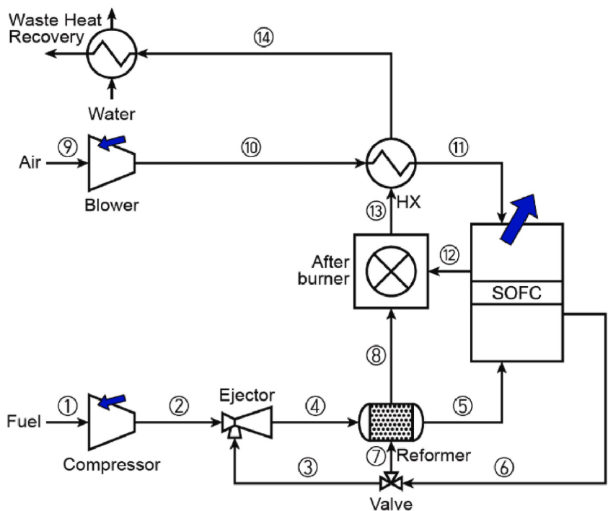
\includegraphics[width=0.9\linewidth]{image1.png}
\caption{Process flow diagram of the baseline Ejector CG layout.}
\label{fig:baseline-ejector-cg}
\end{figure}

Ejector CG is a layout where a portion of anode off -- gas is recirculated as fuel, and the rest is utilized as a hot stream of the reformer.
Air and fuel are pressurized by a blower or compressor to compensate for pressure drop effects and heated in a heat exchanger or reformer before entering the SOFC stack.
By adjusting the split ratio of the three -- way valve, the system can achieve operational flexibility via control of AOGR rate.
The non recirculated part of anode off -- gas flows into the shell side of the reformer to provide heat to the recirculated fuel.
In addition, the remaining heat of both anode and cathode off -- gas can be efficiently utilized by a sequence of raising the temperature of off -- gas mixture through combustion, utilizing the heat at the air heat exchanger, and finally extracting waste heat from the waste heat recovery system.
However, the prior study of Ejector CG layout was conducted for natural gas fueled SOFC system, and operational parameters were not varied.
Since this study analyses ammonia fueled SOFC systems, and operational parameters are varied at a wide range, ejector CG layout has the following limitations.

\begin{enumerate}
\def\labelenumi{\arabic{enumi}.}
\item Depending on system operating conditions, the system may not be thermodynamically feasible.
\item For a given design configuration of a heat exchanger, the required mass flow rate of hot stream at each heat exchanger differs for every single operating condition.
\item Unnecessary parasitic power is induced at the fuel compressor.
\end{enumerate}

An exemplary operating condition when FU = 0.7, anode inlet T = 600\textdegree C, current density = 0.2A/cm\textsuperscript{2}, AOGR ratio = 50\% - which is introduced afterwards as the base case -- is a case where limitation 1 may occur.
The cracking of ammonia is a highly endothermic reaction, hence a large amount of heat duty is required at the reformer.
However, the anode off-gas does not contain sufficient thermal energy to supply heat to the cold stream of the reformer due to its relatively low mass flow rate.
Therefore, in such cases, the thermal energy rich cathode off-gas should be utilized instead as the heat source to supply sufficient heat to the cold stream, while satisfying the 2\textsuperscript{nd} law of thermodynamics.
A T-Q diagram analysis of each cases -- utilizing cathode off-gas as the reformer heat source and anode off-gas as the reformer heat source -- is displayed in the Supplementary Figure S1 to quantitatively verify the need of utilizing cathode off-gas as the heat source of the fuel cracker.

To resolve limitation 2, the heat duty value at both the heat exchanger and reformer must be adjusted to provide a suitable amount of heat to the cold side fluid.
However, the heat duty required at each point differs for every different operating condition of the system.
Since the heat exchanger model and reformer model calculates heat duty and outlet temperature based on design configuration and inlet thermodynamic properties, heat duty can be adjusted by differing the heat exchanger's geometrical parameters or differing the mass flow rate entering the shell side.
Mass flowrate of the shell side fluid greatly affects the amount of heat transfer between the tube and shell side fluid, as a greater mass flowrate substantially increases turbulence in the shell side flow, improving heat transfer performance \cite{ozden2010shell}.
The design configurations of a shell and tube heat exchanger is a unique parameter which cannot be adjusted flexibly in real engineering applications; therefore, shell side inlet mass flowrate is a readily available variable that can be varied.
Shell side inlet mass flowrate can be adjusted by adding a 3-way valve upstream of the heat exchanger and reformer's shell side flow.
The 3-way valve is given a designated split ratio to branch off a suitable mass flowrate of hot gas to the heat exchanger and reformer, so that the cold outlet stream can reach a desired temperature.
In the case of heat exchanger, mass flow rate is branched off to provide a suitable amount of heat for air heating, and in the case of reformer, mass flow rate is branched off to provide a suitable amount of heat for ammonia decomposition and fuel heating.

Limitation 3 occurs due to a difference in the target environment and fuel of the system.
The study conducted by Park~\cite{PARK2023232970} analyzed a natural gas fueled SOFC system for residential heat and power generation, thereby assuming that natural gas is fed into the system at 1 atm.
To induce proper operation at the ejector and compensate for pressure drop effects at the fuel reformer, natural gas is pressurized by the compressor at a high pressure of over 5 atm in the corresponding study.
Such operation causes a significant increase in parasitic power due to power consumption of the fuel compressor.
However, this study considers ammonia as a fuel for marine power generation, where ammonia is conventionally stored at a high pressure of 18 bar for fuel \cite{DNV2023AmmoniaMarineFuelHandbook}.
Therefore, given the sufficiently high inlet pressure of pure ammonia, the fuel compressor is omitted, and a throttling valve is installed instead to meet the required pressure boundary conditions across operating points.
Applying the above three resolutions together, the final process flow diagram of the recirculation system layout is shown in Fig.~\ref{fig:system-layouts-recirc}.

\begin{figure*}[width=\textwidth,pos=!t]
\centering

\begin{subfigure}{0.49\textwidth}
\centering
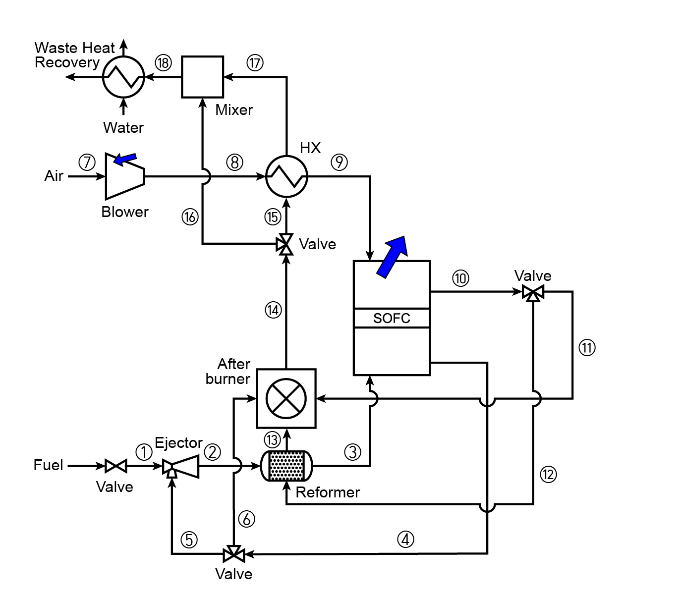
\includegraphics[width=\linewidth]{image3.png}
\caption{}
\label{fig:system-layouts-recirc}
\end{subfigure}%
\hfill
\begin{subfigure}{0.49\textwidth}
\centering
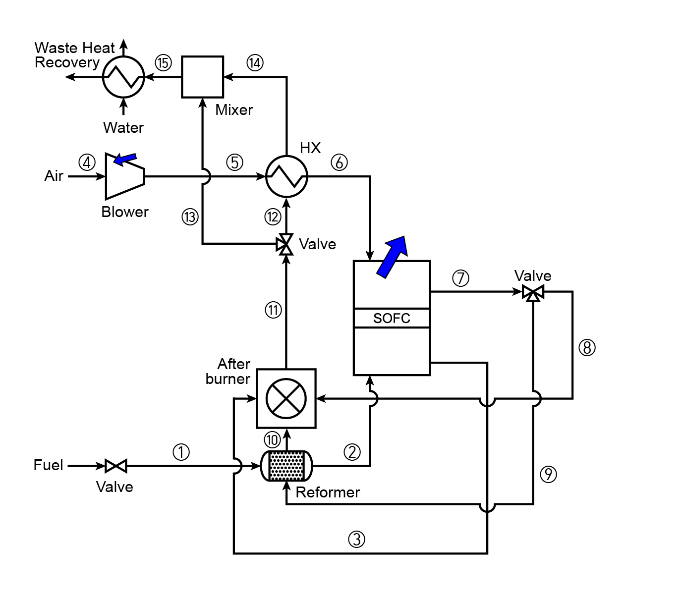
\includegraphics[width=\linewidth]{image2.png}
\caption{}
\label{fig:system-layouts-nonrecirc}
\end{subfigure}%

\caption{System layouts: (a) recirculation system; (b) non-recirculation system.}
\label{fig:system-layouts}
\end{figure*}

\subsubsection{Non-Recirculation System}

In a case where the AOGR ratio is 0, the ejector does not play any role in the system as no part of the anode off -- gas is fed back.
To evaluate non recirculation system performances under unified conditions, an identical system layout was utilized, but the ejector was omitted from the system together with the recirculating 3-way valve.
Since the 3 -- way valve is omitted, all parts of the anode off -- gas is directly fed to the combustor to provide heat to the air heat exchanger after combustion.
The process flow diagram of the non -- recirculation systam layout is shown in Fig.~\ref{fig:system-layouts-nonrecirc}.

\subsection{Input Parameters \& Boundary Conditions}

To compare system performances at different operating conditions, a set of common input parameters must be established to solely analyze the effect of changing operating parameters.
The input parameters and boundary conditions imposed in this study are summarized in Table~\ref{tab:input-params}.
The ambient conditions are set as 25\textdegree C and 1 atm, thereby setting the inlet condition of air as the same temperature and pressure.
Due to the ambient condition, a pressure boundary condition is set at the system sink to be 1 atm, so that neither fluid reflux occurs at the sink nor any unnecessary parasitic power is consumed at the air blower.
In addition, system outlet temperature is set to dew point, as a waste heat recovery system recuperates heat from the exhaust gas until it reaches dew point.
At the fuel inlet side, 100\% ammonia is fed as a saturated vapor at 18 bar, which is the pressure where fully pressurized ammonia is transported and stored as a marine fuel \cite{DNV2023AmmoniaMarineFuelHandbook}.
The temperature of system inlet ammonia is set to 45\textdegree C, which is the saturation temperature of ammonia at 18 bar.
The pressure difference between anode and cathode inlet at the SOFC stack is set to be under 10 mbar to avoid mechanical destruction of the cell \cite{seidler2011pressurized}.
The temperature of the anode and cathode inlet stream is set to be minimum at 600\textdegree C among the parametric study to guarantee complete decomposition of ammonia at the fuel reformer and stack \cite{maffei2008high}.
In addition, the temperature difference between the inlet stream and outlet stream of SOFC stack is set as 100\textdegree C to reduce thermal stress to the stack \cite{cinti2023design}.
The mass flowrate of air through cathode inlet was adjusted at each operating conditions to satisfy the temperature difference boundary condition, as air can be utilized as a coolant to avoid overheating inside the stack.
As fluid flows across the stack, it is assumed that a pressure drop of 0.5\% occurs due to the geometry of anode and cathode channels \cite{LEE2025238271}.

\begin{table}[!t]
\footnotesize
\refstepcounter{table}\label{tab:input-params}%
\noindent\textbf{Table \thetable.} Input parameters and boundary conditions throughout
this study.

\vspace{0.5em}
\footnotesize
\setlength{\tabcolsep}{1.5pt}%
\renewcommand{\arraystretch}{1.35}%
\noindent\begin{tabular}{@{}
  >{\raggedright\arraybackslash}p{(\columnwidth - 6\tabcolsep) * \real{0.582}}
  >{\raggedright\arraybackslash}p{(\columnwidth - 6\tabcolsep) * \real{0.228}}
  >{\raggedright\arraybackslash}p{(\columnwidth - 6\tabcolsep) * \real{0.1335}}
  >{\raggedright\arraybackslash}p{(\columnwidth - 6\tabcolsep) * \real{0.0565}}@{}}
\toprule\noalign{}
\begin{minipage}[b]{\linewidth}\raggedright
Parameter
\end{minipage} & \begin{minipage}[b]{\linewidth}\raggedright
Value
\end{minipage} & \begin{minipage}[b]{\linewidth}\raggedright
Unit
\end{minipage} & \begin{minipage}[b]{\linewidth}\raggedright
Ref.
\end{minipage} \\
\midrule\noalign{}
\textbf{System boundary conditions} & & & \\
System inlet air temperature & 25 & [\textdegree C] & \\
System inlet air pressure & 1 & [atm] & \\
Chemical composition of air & 21\% O\textsubscript{2},
79\% N\textsubscript{2} & [\%] & \\
System inlet fuel temperature & 45 & [\textdegree C] & \cite{DNV2023AmmoniaMarineFuelHandbook}\\
System inlet fuel pressure & 18 & [atm] & \cite{DNV2023AmmoniaMarineFuelHandbook}\\
Chemical composition of fuel & 100\% NH\textsubscript{3} &
[\%] & \\
System sink pressure & 1 & [atm] & \\
System sink temperature & Dew point & [\textdegree C] & \\
\midrule\noalign{}
\textbf{SOFC stack} & & & \\
Number of stacked cells & 2380 & [ea] & \\
Effective cell area & 121 & {[}cm\textsuperscript{2}{]} & \\
Anode pressure drop & 0.5 & [\%] & \cite{LEE2025238271}\\
Cathode pressure drop & 0.5 & [\%] & \cite{LEE2025238271}\\
SOFC inlet pressure difference tolerance & 10 & [mbar] & \cite{seidler2011pressurized}\\
SOFC inlet/outlet temperature difference & 100 & [\textdegree C] & \cite{cinti2023design}\\
\midrule\noalign{}
\textbf{Blower} & & & \\
Isentropic efficiency & 85 & [\%] & \\
\bottomrule\noalign{}
\end{tabular}
\end{table}

The operating conditions of the system analyzed in this system are varied in a wide range with a base case of stack inlet temperature 600\textdegree C (\(T_{stack})\),stack fuel utilization rate 70\% (\({FU}_{stack}\)), current density 0.2A/cm\textsuperscript{2} (\emph{j}), AOGR ratio 50\% (\emph{r}), which is a condition to generate approximately 50 kW of gross power.
To meet the power demand under given operating conditions, the SOFC stack is consisted of 2380 cells with an active area of 121cm\textsuperscript{2}.
Along with the scale of SOFC stack, mass flow rates of fuel inlet at each operating condition is determined as the following equations.

\begin{align}
\begin{split}
{\dot{m}}_{{NH}_{3}} &= \frac{2{\dot{n}}_{O^{2 -}}{MW}_{{NH}_{3}}}{3{FU}_{stack}} \\
&\quad \cdot \left( 1 - r\left( 1 - {FU}_{stack} \right) \right)
\end{split} \label{eq:fuel-flow} \\
{\dot{n}}_{O^{2 -}} &= \frac{jN_{cell}A_{cell}}{2F} \label{eq:ion-transport}
\end{align}

Where \({\dot{n}}_{O^{2 -}}\) is the rate of oxygen ion transport,
\({MW}_{{NH}_{3}}\) is the molar mass of ammonia, respectively. When
AOGR is applied, unused fuel from the SOFC stack outlet is recirculated, and the recirculated fuel supplies the fuel demand at the anode inlet.
Such process reduces the amount of fuel required at the system inlet to satisfy \({FU}_{stack}\) conditions.

Dimensional parameters for the heat exchanger and reformer were determined following standard design guidelines for commercial shell-and-tube heat exchangers \cite{thulukkanam2000heat,kakacc2002heat, thome2006wolverine}.
Key geometric variables---including tube length, shell diameter, and baffle spacing---were tuned to ensure that the required heat duties are met over a wide operating range.
To prevent overdesign, the final dimensions were selected such that the tube-side velocity remained within an appropriate range for effective heat transfer.
However, since fluid flow rates vary substantially across operating conditions, a single heat exchanger design cannot staisfy the heat duty and velocity requirements at every point, even with three-way valve fluid control.
Therefore, if a given heat exchanger unit could not physically meet its heat duty requirements or tube-side velocity range, its size would be adjusted to meet such conditions.
The main geometric parameters of the base-case heat exchanger and reformer are summarized in Table~\ref{tab:hx-reformer-design}.

\begin{table}[!t]
\footnotesize
\refstepcounter{table}\label{tab:hx-reformer-design}%
\noindent\textbf{Table \thetable.} Heat exchanger \& reformer design configurations for
base case operation

\vspace{0.5em}
\footnotesize
\setlength{\tabcolsep}{1.5pt}%
\renewcommand{\arraystretch}{1.35}%
\noindent\begin{tabular}{@{}
  >{\raggedright\arraybackslash}p{(\columnwidth - 6\tabcolsep) * \real{0.582}}
  >{\raggedright\arraybackslash}p{(\columnwidth - 6\tabcolsep) * \real{0.228}}
  >{\raggedright\arraybackslash}p{(\columnwidth - 6\tabcolsep) * \real{0.1335}}
  >{\raggedright\arraybackslash}p{(\columnwidth - 6\tabcolsep) * \real{0.0565}}@{}}
\toprule\noalign{}
\begin{minipage}[b]{\linewidth}\raggedright
Parameter
\end{minipage} & \begin{minipage}[b]{\linewidth}\raggedright
Value
\end{minipage} & \begin{minipage}[b]{\linewidth}\raggedright
Unit
\end{minipage} & \begin{minipage}[b]{\linewidth}\raggedright
Ref.
\end{minipage} \\
\midrule\noalign{}
\textbf{Air heat exchanger} & & & \\
Shell diameter & 0.643 & [m] & \cite{thulukkanam2000heat}\\
Tube diameter & 0.0127 & [m] & \\
Number of tubes & 945 & [ea] & \\
Baffle spacing & 0.214 & [m] & \\
\midrule\noalign{}
\textbf{Ammonia reformer} & & & \\
Shell diameter & 0.308 & [m] & \cite{thulukkanam2000heat}\\
Tube diameter & 0.0127 & [m] & \\
Number of tubes & 134 & [ea] & \\
Baffle spacing & 0.103 & [m] & \\
Catalyst pellet diameter & 0.002974 & [m] & \\
Catalyst pellet length & 0.01041 & [m] & \\
\bottomrule\noalign{}
\end{tabular}
\end{table}

\subsection{Operating parameters for parametric study}

To analyze the operating limits and performance effects of AOGR ratio via parametric study, the following operating parameters were varied together with AOGR ratio: \(T_{stack}\), \({FU}_{stack}\), \emph{j}.
The range and values of parameter variation are described in Table~\ref{tab:operating-params}.

\begin{table}[!t]
\footnotesize
\refstepcounter{table}\label{tab:operating-params}%
\noindent\textbf{Table \thetable.} Variations in the operating parameters.

\vspace{0.5em}
\footnotesize
\setlength{\tabcolsep}{1.5pt}%
\renewcommand{\arraystretch}{1.35}%
\noindent\begin{tabular}{@{}
  >{\raggedright\arraybackslash}p{(\columnwidth - 4\tabcolsep) * \real{0.38}}
  >{\raggedright\arraybackslash}p{(\columnwidth - 4\tabcolsep) * \real{0.44}}
  >{\raggedright\arraybackslash}p{(\columnwidth - 4\tabcolsep) * \real{0.18}}@{}}
\toprule\noalign{}
\begin{minipage}[b]{\linewidth}\raggedright
Operating parameters
\end{minipage} & \begin{minipage}[b]{\linewidth}\raggedright
Values
\end{minipage} & \begin{minipage}[b]{\linewidth}\raggedright
Unit
\end{minipage} \\
\midrule\noalign{}
\(T_{stack}\) & 600, 650, 700, 750, 800 & [\textdegree C] \\
\({FU}_{stack}\) & 40, 50, 60, 70, 80 & [\%] \\
\emph{j} & 0.1, 0.2, 0.3, 0.4, 0.5 &
{[}A/cm\textsuperscript{2}{]} \\
AOGR ratio & 0, 10, 20, 30, 40, 50\ldots{} Max & [\%] \\
\bottomrule\noalign{}
\end{tabular}
\end{table}

\FloatBarrier

\section{Results and Discussion}

To analyze the sole effect of each operating parameter, each parameters were primarily varied at the base case.
The complete stream table for the base case operation is provided in supplementary table XX.
Key performance indices include system gross power, electrical efficiency, etc.
In this study, the only parasitic power induced in the system is power consumption at the air blower.
Therefore, electrical efficiency and net power can be defined as Eqs.~\eqref{eq:efficiency} and \eqref{eq:net-power}.
To evaluate the performance of the system's capability to generate electrical power at a non-biased scale, the gross power was normalized as power density, defined as Eq.~\eqref{eq:power-density}.

\begin{align}
\eta_{elec} &= \frac{\dot{W}_{net}}{\dot{n}_{fuel} LHV_{fuel}} \times 100, \label{eq:efficiency} \\
\dot{W}_{net} &= \dot{W}_{gross} - \dot{W}_{blower}, \label{eq:net-power} \\
\dot{w}_{gross} &= \frac{\dot{W}_{gross}}{N_{cell} A_{cell}}. \label{eq:power-density}
\end{align}

\subsection{Determination of maximum AOGR Ratio}

In the system layout proposed in this study, maximum AOGR ratio is limited by fluid properties of the anode side gas.
To inspect in detail the mechanism of determination of maximum AOGR ratio, the streams of the anode side gas and its recirculated portion can be detached from the overall system to compose an AOGR loop section as Fig.~\ref{fig:aogr-loop}.

\begin{figure*}[width=\textwidth,pos=!t]
\centering
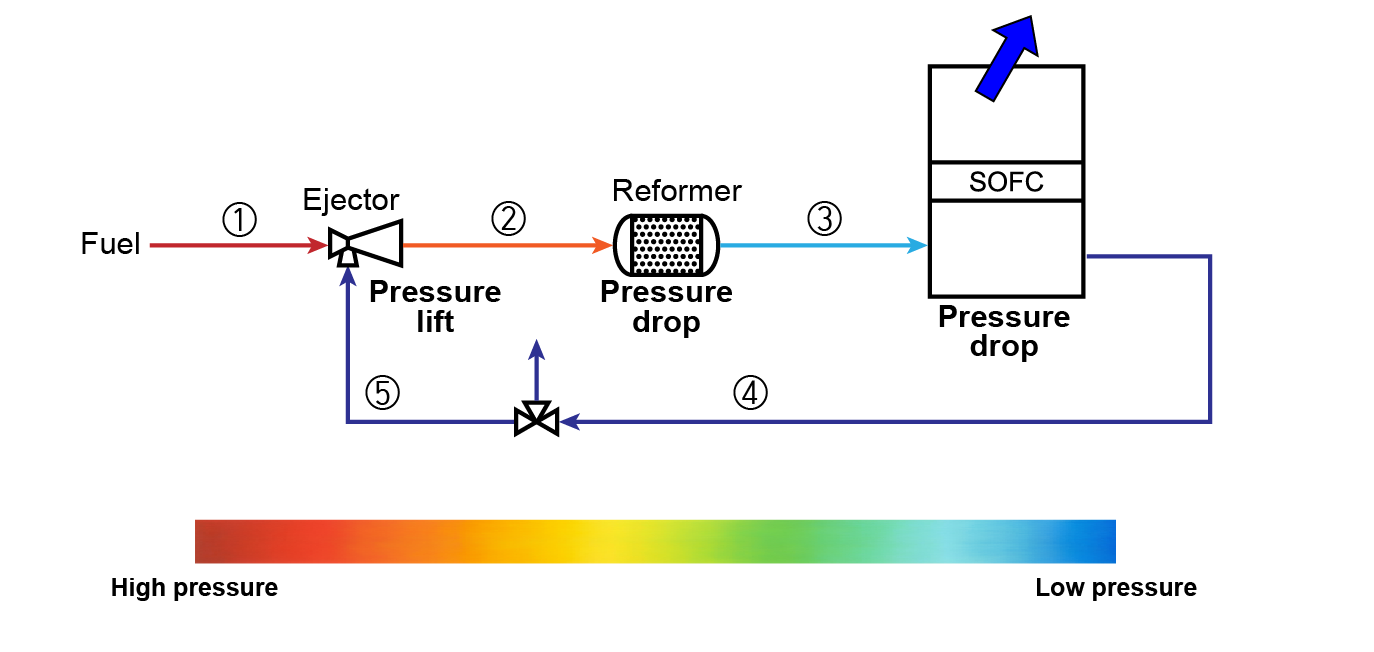
\includegraphics[width=0.75\linewidth]{image4.png}
\caption{Schematic diagram of the AOGR loop section and pressure distribution in the constituent streams.}
\label{fig:aogr-loop}
\end{figure*}

As a mixture of system inlet fuel and the recirculated portion of anode off - gas (stream 2) flows consecutively through the fuel reformer and stack anode channel, the stream undergoes pressure drop and exits the stack (stream 4).
A portion of the low-pressure anode off -- gas is branched off through the three-way valve depending on the AOGR ratio (stream 5) and enters the suction inlet of the ejector.
The pressure of stream 5 must be elevated to compensate for pressure drop effects of the fuel reformer and stack anode channel.
Therefore, a high-pressure fuel (stream 1) enters through the primary inlet of the ejector and is mixed with stream 5 to pressurize the recirculated fluid.
The mixed fluid leaves the ejector at a back pressure as stream 2, and the pressure balance of AOGR loop is satisfied.

As the system AOGR ratio increases, the entrainment ratio of the ejector also increases.
Under this condition, a larger mass flow rate of the low-pressure fluid in stream 5 is entrained into the ejector, and therefore the pressure of stream 1 must be increased to ensure proper mixing with stream 5 and to achieve the desired back pressure at stream 2.
This is because a higher primary inlet pressure increases the stagnation pressure of the primary flow, thereby supplying more kinetic energy to the mixed fluid and resulting in greater pressure recovery \cite{wang2017experimental}.
However, the maximum pressure of stream 1 is limited to 18 bar, and the 18 bar primary flow may not be able to sufficiently pressurize the recirculated stream when the AOGR ratio is too high.
In addition to this, the pressure drop occurring at the fuel cracker cold side also generally increases with the AOGR ratio due to an increase in the mass flowrate of stream 2.
Therefore, it can be deduced that the maximum AOGR ratio of the system is determined by the following two factors: entrainment and pressurization performance of the ejector, and pressure drop occurring at the fuel reformer cold side.

Changes in operating conditions of the SOFC system (\({FU}_{stack}\), \emph{j}, \(T_{stack}\)) can affect both the performance of the ejector and fuel reformer cold side pressure drop.
Therefore, it is necessary to analyze how a change in each operating condition affects the maximum AOGR ratio permitted to the system.

In the case of \({FU}_{stack}\), its value directly determines the ammonia fuel flow rate supplied to the system inlet, thereby strongly affecting the mass flow rate of anode-side gases.
As \({FU}_{stack}\) increases from 40\% to 80\%, the ammonia fuel flow rate required to sustain the target electrochemical operating condition of the SOFC stack decreases, which in turn reduces the mass flow rate of the anode-side gases passing through the fuel cracker cold side.
For a given packed bed reformer geometry, this reduction in flow rate diminishes the viscous friction effect within the catalyst bed, leading to a decrease in the cold side pressure drop.
As shown in Fig.~\ref{fig:max-aogr}(a), when \({FU}_{stack}\) increases from 40\% to 80\%, the reformer cold side pressure drop decreases monotonically from 8.76 kPa at 40\% \({FU}_{stack}\) to 6.66 kPa at 80\% \({FU}_{stack}\).
Since a lower reformer cold-side pressure drop alleviates the discharge back pressure of the ejector imposed in the AOGR loop, the maximum allowable AOGR ratio that the system can sustain correspondingly increases from 65.4\% to 66.9\% over the same \({FU}_{stack}\) range.
This trend indicates that operating the system at higher \({FU}_{stack}\) is operationally favorable for expanding the feasible AOGR operating window, as the reduced anode-side flow rate mitigates the parasitic pressure losses across the reformer and thereby relaxes the pressure-balance constraint that governs the upper bound of the AOGR ratio.

In the case of \emph{j}, its value directly determines the amount of fuel electrochemically consumed in the SOFC stack, and thereby simultaneously increases both the air and ammonia fuel flow rates required at the system inlet.
As \emph{j} increases from 0.1 A/cm\textsuperscript{2} to 0.5 A/cm\textsuperscript{2}, the ammonia fuel flow rate required to sustain the elevated electrochemical reaction rate rises accordingly, which in turn increases the mass flow rate of the anode-side gases passing through the fuel cracker cold side.
Furthermore, a higher \emph{j} leads to a larger heat duty for the endothermic ammonia decomposition reaction, which requires a longer fuel cracker length to provide sufficient heat transfer area.
The combined effect of the increased flow rate and the extended cracker length amplifies the viscous friction loss along the packed catalyst bed, leading to a substantial increase in the cold side pressure drop.
As shown in Fig.~\ref{fig:max-aogr}(b), when \emph{j} increases from 0.1 A/cm\textsuperscript{2} to 0.5 A/cm\textsuperscript{2}, the reformer cold side pressure drop increases monotonically from 6.50 kPa at 0.1 A/cm\textsuperscript{2} to 11.14 kPa at 0.5 A/cm\textsuperscript{2}.
Since a higher cracker cold-side pressure drop intensifies the discharge back pressure of the ejector imposed in the AOGR loop, the maximum allowable AOGR ratio that the system can sustain correspondingly decreases from 67.3\% to 62.0\% over the same \emph{j} range.
This trend indicates that operating the system at higher \emph{j} narrows the feasible AOGR operating window, as the simultaneous increase in anode-side flow rate and reformer length aggravates the parasitic pressure losses across the cracker and thereby tightens the pressure-balance constraint that governs the upper bound of the AOGR ratio.

In the case of \(T_{stack}\), its value directly determines the temperature of the entrained anode off-gas returning to the ejector as well as the temperature of the gas entering the fuel cracker cold side.
As \(T_{stack}\) increases from 600 \textdegree C to 800 \textdegree C, the elevated gas temperature reduces the gas density at a fixed mass flow rate, which in turn increases the volumetric flow velocity through the fuel cracker cold side.
This higher flow velocity enhances the viscous friction loss along the packed catalyst bed, leading to a gradual increase in the cold side pressure drop.
As shown in Fig.~\ref{fig:max-aogr}(c), when \(T_{stack}\) increases from 600 \textdegree C to 800 \textdegree C, the reformer cold side pressure drop increases monotonically from 6.96 kPa at 600 \textdegree C to 8.66 kPa at 800 \textdegree C.
However, in contrast to the cases of \({FU}_{stack}\) and \emph{j}, the variation in the cold side pressure drop alone is insufficient to account for the magnitude of the change in the maximum allowable AOGR ratio, which decreases from 66.6\% at 600 \textdegree C to 61.2\% at 800 \textdegree C over the same temperature range.
Such substantial reduction implies that, under varying \(T_{stack}\), the upper bound of the AOGR ratio is governed not only by the reformer pressure drop but more dominantly by the entrainment performance of the ejector itself.

Specifically, as the temperature of the entrained anode off-gas rises while the primary flow condition remains fixed, the speed of sound of the secondary stream also increases, which leads to a reduction in the convective Mach number that characterizes the compressible mixing process between the primary and secondary flows within the ejector.
According to the recent numerical investigation of supersonic ejector mixing by Liang et al.~\cite{liang2025numerical} a lower convective Mach number---corresponding to a higher total temperature ratio between the secondary and primary flows---weakens the momentum exchange across the confined mixing layer, thereby deteriorating the mixing process between the two streams.
Since insufficient mixing prevents the secondary flow from being adequately accelerated by the high-velocity primary flow, the Mach number of the mixed flow at the diffuser inlet decreases, which in turn degrades both the entrainment capability and the pressure lift performance of the ejector.
Consequently, the ejector becomes less capable of overcoming the discharge back pressure of the AOGR loop, and the maximum allowable AOGR ratio decreases more sharply than what the reformer pressure drop alone would predict.
To verify this, a supplementary analysis was conducted by modelling a simple ejector system inhaling pure ammonia as primary flow and arbitrary anode off-gas as the entrained flow.
The results confirm that for a constant entrainment ratio, pressure lift performance of the ejector decreases as the temperature of entrainment flow increases (Supplementary Table XX).
This trend indicates that operating the system at higher \(T_{stack}\) is operationally unfavorable for sustaining a wide AOGR operating window, as the deteriorated performance becomes the dominant constraint that governs the upper bound of the AOGR ratio.

\begin{figure*}[width=\textwidth,pos=!t]
\centering
\begin{subfigure}{0.33\linewidth}
\centering
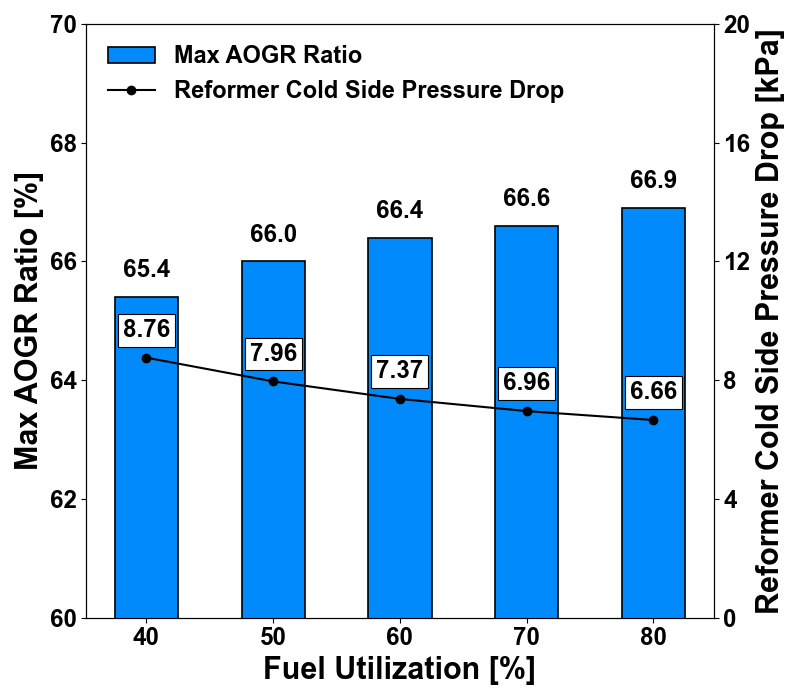
\includegraphics[width=\linewidth]{image5.png}
\caption{}
\end{subfigure}%
\hfill
\begin{subfigure}{0.33\linewidth}
\centering
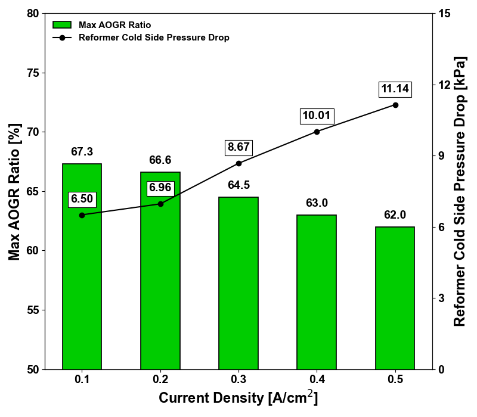
\includegraphics[width=\linewidth]{image6.png}
\caption{}
\end{subfigure}%
\hfill
\begin{subfigure}{0.33\linewidth}
\centering
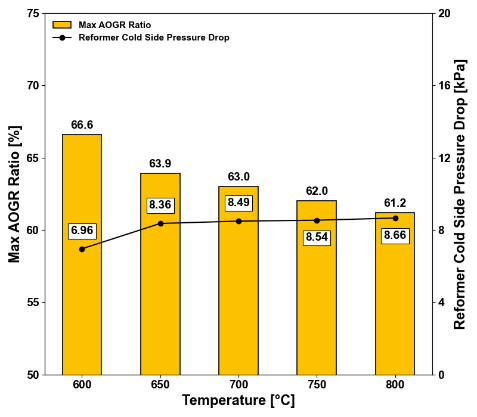
\includegraphics[width=\linewidth]{image7.png}
\caption{}
\end{subfigure}%
\caption{Maximum AOGR ratio permitted for variations in (a) \({FU}_{stack}\), (b) \emph{j}, and (c) \(T_{stack}\).}
\label{fig:max-aogr}
\end{figure*}

\subsection{Effect of AOGR ratio at different operating conditions}

While the previous section identified the maximum allowable AOGR ratio under each operating condition, the AOGR ratio itself is a key design variable that strongly influences the overall system performance within the feasible operating window.
In this section, the effect of the AOGR ratio on the system performance is investigated under varying operating conditions, namely \({FU}_{stack}\), \emph{j}, and \(T_{stack}\).
For each operating condition, the AOGR ratio is varied from zero up to the maximum allowable value determined in Section 4.1, and the resulting trends in system efficiency and key state variables are analyzed.
This two-dimensional parametric analysis enables a comprehensive understanding of how the AOGR ratio interacts with each operating condition to shape the overall performance characteristics of the NH$_3$-fueled SOFC system.

\subsubsection{Effect of AOGR ratio at different fuel utilizations}

To investigate the influence of the AOGR ratio on the system performance under varying \({FU}_{stack}\), the AOGR ratio was swept from 0\% up to the maximum allowable value identified in Section 4.1, while \({FU}_{stack}\) was varied from 40\% to 80\%.
The resulting trends in system efficiency and stack power density are summarized in Fig.~\ref{fig:fuel-utilization-map}(a), where each iso-fuel-utilization line traces the trajectory of the system operating point as the AOGR ratio increases.

As shown in Fig.~\ref{fig:fuel-utilization-map}(a), increasing the AOGR ratio consistently improves system efficiency while reducing stack power density across all \({FU}_{stack}\) conditions.
However, these two opposing effects respond differently to \({FU}_{stack}\): the efficiency gain varies significantly with \({FU}_{stack}\), whereas the power density penalty remains nearly insensitive to it.
At a low \({FU}_{stack}\) of 40\%, raising the AOGR ratio from 0\% to its maximum allowable value of 65.4\% increases the system efficiency from 33.9\% to 51.3\%, an absolute gain of 17.4 percentage points.
At a high \({FU}_{stack}\) of 80\%, the same operation only improves the efficiency from 64.5\% to 68.0\%, yielding a much smaller gain of 3.5 percentage points.
This asymmetry indicates that the efficiency benefit of AOGR is substantially greater at low \({FU}_{stack}\).

The origin of this asymmetry can be explained by the AOGR-induced reduction in the system fuel input.
Under steady-state operation, the mass flow rate of ammonia required at the system inlet to sustain a target \({FU}_{stack}\) is given by Eq.~\eqref{eq:fuel-flow}.

The first parenthetical term on the right-hand side represents the stoichiometric fuel consumption rate, while the second term,
\(\left( 1 - r(1 - FU_{stack}) \right)\), captures the effect of AOGR on the system-level fuel demand.
Since
\(\left( 1-FU_{stack} \right)\)is the unutilized fuel fraction exiting
the stack, the term \(r(1 - FU_{stack})\) quantifies the amount of unreacted fuel recovered through recirculation.
At low \({FU}_{stack}\), a substantial fraction of unreacted fuel is available for recovery, so even modest AOGR ratios significantly reduce the fresh fuel demand.
At high \({FU}_{stack}\), the recoverable amount is limited and AOGR provides only marginal savings.
As shown in Fig.~\ref{fig:fuel-utilization-map}(b), at \({FU}_{stack}\) = 40\% the system fuel input expressed in terms of thermal energy decreases dramatically from 157.6 kW to 95.7 kW, whereas at \({FU}_{stack}\) = 80\% it decreases only from 78.8 kW to 68.2 kW---a disparity that directly translates into the efficiency gain disparity observed in Fig.~\ref{fig:fuel-utilization-map}(a).

In contrast, the stack power density penalty associated with AOGR is nearly independent of \({FU}_{stack}\).
As the AOGR ratio increases, the recirculated stream---rich in N$_2$ and H$_2$O---dilutes the fresh decomposed fuel and lowers the hydrogen partial pressure at the stack anode inlet.
According to the Nernst equation, this reduction suppresses the open circuit voltage (OCV) and consequently the cell voltage.
As shown in Fig.~\ref{fig:fuel-utilization-map}(c), increasing the AOGR ratio from 0\% to its maximum value reduces the cell voltage from 0.941 V to 0.878 V at \({FU}_{stack}\) = 40\% (a drop of 0.063 V), and from 0.903 V to 0.832 V at \({FU}_{stack}\) = 80\% (a drop of 0.071 V).
The two voltage drops differ by less than 10 mV, indicating that the AOGR-induced voltage degradation is essentially comparable across the \({FU}_{stack}\) range.
This near-uniform behavior arises because the fuel dilution effect due to AOGR occurs in a similar magnitude among different \({FU}_{stack}\) values.
Consistent with this, the resulting power density reductions---from 0.188 W/cm\textsuperscript{2} to 0.176 W/cm\textsuperscript{2} at FU = 40\% and from 0.181 W/cm\textsuperscript{2} to 0.166 W/cm\textsuperscript{2} at FU = 80\%---differ by only 0.003 W/cm\textsuperscript{2}.
Such results show that AOGR is most advantageous for SOFC systems operated at relatively low \({FU}_{stack}\).

\begin{figure*}[width=\textwidth,pos=!t]
\centering
\begin{subfigure}{0.49\linewidth}
\centering
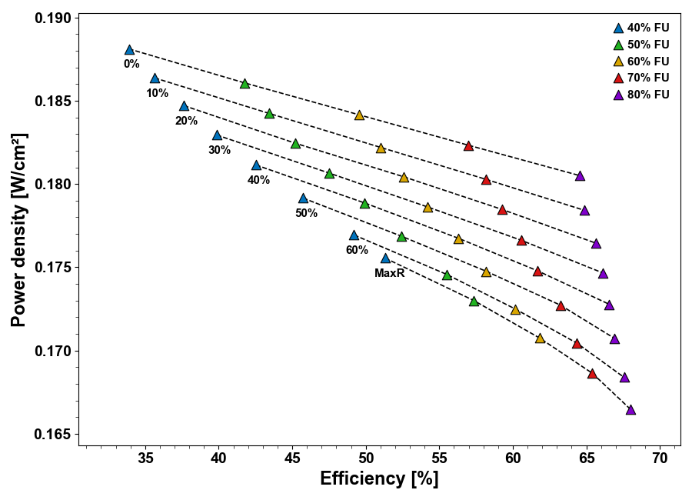
\includegraphics[width=\linewidth]{image8.png}
\caption{}
\end{subfigure}%
\hfill
\begin{subfigure}{0.49\linewidth}
\centering
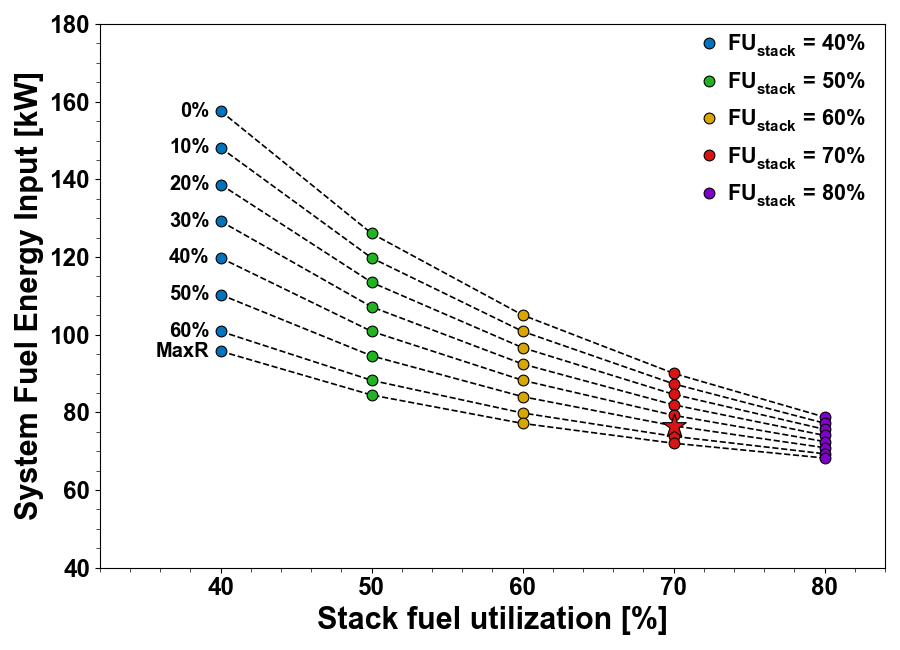
\includegraphics[width=\linewidth]{image9.png}
\caption{}
\end{subfigure}%
\par\medskip
\begin{subfigure}{0.49\linewidth}
\centering
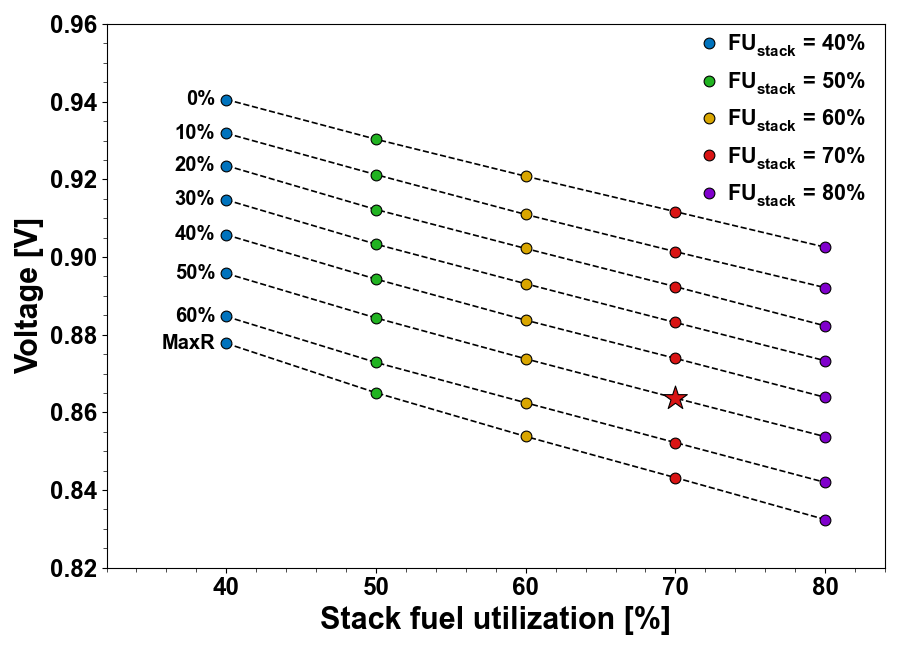
\includegraphics[width=\linewidth]{image10.png}
\caption{}
\end{subfigure}%
\caption{Performance map showing (a) efficiency and power density, (b) LHV, and (c) voltage as a function of \({FU}_{stack}\) and AOGR ratio.}
\label{fig:fuel-utilization-map}
\end{figure*}

\subsubsection{Effect of AOGR ratio at different current density}

System performance was next examined under varying \emph{j} and AOGR ratio, and the resulting trajectories of system efficiency and stack power density are presented in Fig.~\ref{fig:current-density-map}(a).
At a low \emph{j} of 0.1 A/cm\textsuperscript{2}, increasing the AOGR ratio from 0\% to its maximum allowable value of 67.3\% improves the system efficiency from 60.7\% to 69.9\%, corresponding to an absolute gain of 9.2 percentage points.
At a high \emph{j} of 0.5 A/cm\textsuperscript{2}, however, the same operation only enhances the efficiency from 46.3\% to 49.8\%, yielding a much smaller gain of 3.5 percentage points.
Notably, the iso-\emph{j} trajectories at high \emph{j} exhibit a non-monotonic behavior: at 0.5 A/cm\textsuperscript{2}, the system efficiency increases with the AOGR ratio up to approximately 60\%, but then decreases as the AOGR ratio is further raised toward its maximum allowable value.
The existence of an internal optimum at high \emph{j} indicates that AOGR introduces a competing penalty that becomes increasingly dominant as \emph{j} increases.

In contrast, the trend in stack power density with increasing AOGR ratio is far less sensitive to \emph{j}.
As shown in Fig.~\ref{fig:current-density-map}(b), the cell voltage at any given \emph{j} decreases by a comparable magnitude as the AOGR ratio is increased, regardless of the absolute \emph{j} level.
Specifically, increasing the AOGR ratio from 0\% to its maximum value reduces the cell voltage from 0.962 V to 0.890 V at 0.1 A/cm\textsuperscript{2} (a drop of 0.072 V) and from 0.790 V to 0.732 V at 0.5 A/cm\textsuperscript{2} (a drop of 0.058 V).
The slightly larger voltage drop observed at low \emph{j} is partly attributable to the significantly wider AOGR sweep range, since the maximum allowable AOGR ratio is 67.3\% at 0.1 A/cm\textsuperscript{2} but only 62.0\% at 0.5 A/cm\textsuperscript{2}.
When this difference in the AOGR sweep range is taken into account, the corresponding relative reductions in power density---from 0.096 W/cm\textsuperscript{2} to 0.089 W/cm\textsuperscript{2} at 0.1 A/cm\textsuperscript{2} and from 0.395 W/cm\textsuperscript{2} to 0.366 W/cm\textsuperscript{2} at 0.5 A/cm\textsuperscript{2}---correspond to nearly the same value of approximately 7\% in both cases.
This near-uniform power density degradation across \emph{j} conditions can be understood from the fact that \emph{j} does not significantly alter the molar composition at the stack inlet and outlet.
Consequently, the resulting reduction in the anode hydrogen partial pressure is governed primarily by the AOGR ratio itself rather than by the operating \emph{j}.
Since the power density penalty alone cannot account for the non-monotonic efficiency behavior observed at high \emph{j}, the source of the reversal must instead lie in the parasitic power consumption of the system BoP.

\begin{figure*}[width=\textwidth,pos=!t]
\centering
\begin{subfigure}{0.49\linewidth}
\centering
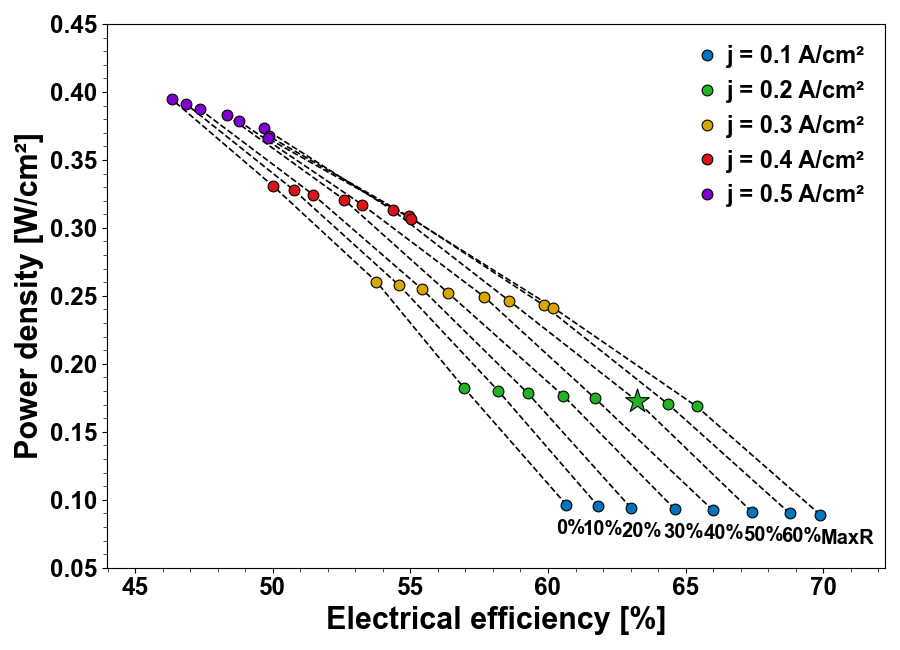
\includegraphics[width=\linewidth]{image11.png}
\caption{}
\end{subfigure}%
\hfill
\begin{subfigure}{0.49\linewidth}
\centering
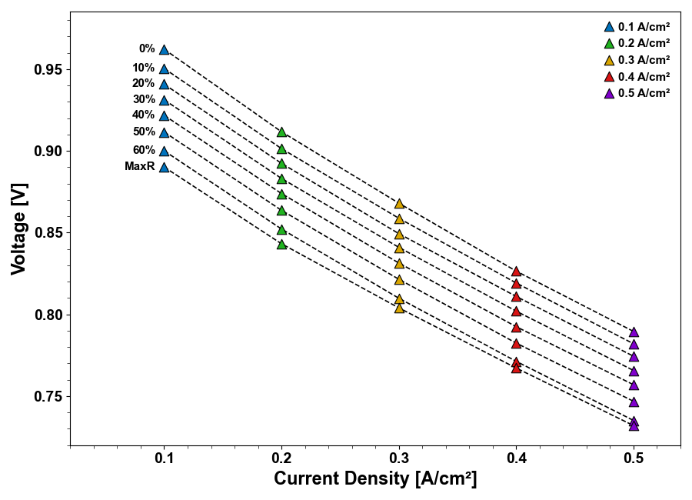
\includegraphics[width=\linewidth]{image12.png}
\caption{}
\end{subfigure}%
\caption{Performance map showing (a) efficiency and power density and (b) voltage as a function of \emph{j} and AOGR ratio.}
\label{fig:current-density-map}
\end{figure*}

To clarify this, the system parasitic power was taken into analysis.
As addressed in Eq.~\eqref{eq:net-power}, the air blower is responsible for parasitic power consumption in the present system, and the pressure rise that the air blower must provide is determined by the cumulative pressure drop along the cathode-side flow path, given by Eq.~\eqref{eq:blower-pressure}.

\begin{equation}
\begin{split}
p_{air\,blower} = 1\,\mathrm{atm} &+ \Delta p_{stack} + \Delta p_{cracker,hot} \\
&+ \Delta p_{air\,HX,hot}.
\end{split}
\label{eq:blower-pressure}
\end{equation}

where \(\Delta p_{stack}\) is the pressure drop across the SOFC stack cathode channel, \(\Delta p_{cracker,hot}\) is the pressure drop across the hot side of the fuel cracker, and \(\Delta p_{air\,HX,hot}\) is the pressure drop across the hot side of the air heat exchanger.
The flow path of fluid to be pressurized by the air blower is represented in supplementary figure XX.
As AOGR ratio increases, the pressure drops occurring at the heat exchanger and fuel cracker are amplified, while the SOFC stack channel pressure dop is determined almost constant as 0.5\% of the fluid pressure.
First, the pressure drop on the hot side of the fuel cracker rises through a more subtle mechanism than a simple increase in the cold-side flow rate.
With increasing AOGR ratio, the mass flow rate of fresh ammonia entering the cracker cold inlet decreases, since a larger fraction of the stack inlet fuel demand is met by recirculated unreacted fuel.
This reduction in ammonia content moderately lowers the heat duty required for the endothermic NH$_3$ decomposition reaction.
However, the AOGR ratio simultaneously raises the temperature of the cracker cold inlet stream, because the recirculated anode off-gas---returning at a high temperature---constitutes an increasingly large fraction of the cold stream.
Since the cracker hot stream inlet temperature is essentially fixed as the stack cathode off gas temperature, the elevated cold-side temperature causes the log-mean temperature difference (LMTD) across the cracker to decrease substantially.
Because the LMTD reduction outweighs the moderate decrease in the heat duty, the mass flow rate of the hot stream required to satisfy the heat balance must increase, leading to a higher pressure drop \(\Delta p_{Cracker,hot}\)on the hot side of the fuel cracker.
The corresponding data of LMTD and heat duty at the fuel cracker is provided in supplementary table XX for different AOGR ratio operation.
Second, the pressure drop on the hot side of the air heat exchanger rises through a chain of effects originating from the stack inlet-outlet temperature difference boundary condition.
In SOFC operation, the cathode air flow rate is determined by the boundary condition that the temperature difference between the stack inlet and outlet must remain at 100\textdegree C.
As discussed earlier, increasing the AOGR ratio reduces the cell operating voltage and consequently lowers the stack power generation.
Since the total chemical energy released by the electrochemical reaction is partitioned between electrical work and heat, a reduction in the electrical power output translates directly into an increase in the heat that must be removed from the anode to maintain the prescribed inlet--outlet temperature difference.
To dissipate this additional heat, the cathode air flow rate must therefore be increased.
This larger air flow rate elevates the heat capacity flow rate (\(\dot{m}C_{p}\)) on the cold side of the air heat exchanger, which receives the cathode air at ambient temperature and heats it up to \(T_{stack}\).
Since the cold stream now carries a greater thermal load to be transferred from the hot stream, and since the cold-side outlet temperature must remain fixed at the \(T_{stack}\) setpoint, the mass flow rate of the hot stream supplying the air heat exchanger must also increase to satisfy the heat balance.
Consequently, \(\Delta p_{air\text{\,}HX,hot}\) grows with the AOGR ratio.
Combined with the direct increase in air flow rate through the blower itself, these compounding effects cause the air blower parasitic power to grow rapidly with the AOGR ratio.

The relative impact of this parasitic power growth on the overall system efficiency depends strongly on the operating \emph{j}, since the absolute magnitude of both air flow rate and pressure drops occurring at the heat exchanger and fuel cracker scales with \emph{j}.
As summarized in Table~\ref{tab:parasitic-power}, at a low \emph{j} of 0.1 A/cm\textsuperscript{2}, the air blower parasitic power increases from 0.31 kW at zero recirculation to 0.52 kW at the maximum AOGR ratio, accompanied by an increase in \(\Delta p_{Cracker,hot}\)from 1.83 kPa to 3.20 kPa and in
\(\Delta p_{air\text{\,}HX,hot}\)from 1.92 kPa to 3.04 kPa. 
Although the absolute increase in parasitic power ($\approx$210 W) is non-negligible, it remains a minor fraction of the gross stack power output, corresponding to approximately 1\% of the gross power generated under this operating condition.
As a result, at low \emph{j} the efficiency gain from reduced fuel input clearly dominates over the parasitic penalty, and the efficiency increases monotonically with the AOGR ratio.
At a high \emph{j} of 0.5 A/cm\textsuperscript{2}, in contrast, the air blower parasitic power soars from 9.42 kW at zero recirculation to 14.13 kW at the maximum AOGR ratio---an absolute increase of approximately 22 times larger than the low-\emph{j} case.
The associated pressure drops on the hot side of the fuel cracker and the air heat exchanger also rise much more steeply, from 4.15 kPa to 9.93 kPa and from 12.04 kPa to 14.68 kPa, respectively.
The increase in parasitic power at this condition reaches approximately 4.5\% of the gross stack power output at the maximum AOGR ratio, which is significant enough to overcome the benefit of reduced fuel input beyond a certain AOGR ratio.
Consequently, at 0.5 A/cm\textsuperscript{2}, the system efficiency continues to improve only up to about 60\% AOGR; beyond this point, the marginal increase in parasitic power exceeds the marginal reduction in fuel input, and the efficiency begins to decline despite the continued recovery of unutilized fuel.
As a result, the dominant trade-off under varying \emph{j} shifts from the stack level to the balance-of-plant level, such that the optimal AOGR ratio at high \emph{j} lies below the maximum allowable value and decreases further as \emph{j} increases.

\begin{table*}[!t]
\footnotesize
\refstepcounter{table}\label{tab:parasitic-power}%
\noindent\textbf{Table \thetable.} Summary of parasitic power and pressure drops for different AOGR ratios at different \emph{j} values

\vspace{0.5em}
\small
\setlength{\tabcolsep}{2pt}%
\renewcommand{\arraystretch}{1.35}%
\noindent\begin{tabular*}{\textwidth}{@{\extracolsep{\fill}}l cc cc cc cc cc c@{}}
\toprule\noalign{}
Parameters & \multicolumn{10}{c}{Values} & Units \\
\midrule\noalign{}
\emph{j} & \multicolumn{2}{c}{0.1} & \multicolumn{2}{c}{0.2} & \multicolumn{2}{c}{0.3} & \multicolumn{2}{c}{0.4} & \multicolumn{2}{c}{0.5} & A/cm\textsuperscript{2} \\
\cmidrule{2-11}
AOGR ratio & 0 & Max & 0 & Max & 0 & Max & 0 & Max & 0 & Max & \% \\
\midrule\noalign{}
\(\Delta p_{cracker,\,hot}\) & 1.83 & 3.20 & 2.50 & 3.89 & 3.21 & 6.01 & 3.32 & 8.01 & 4.15 & 9.93 & kPa \\
\(\Delta p_{air\,HX,\,hot}\) & 1.92 & 3.04 & 3.49 & 3.69 & 5.23 & 6.69 & 8.32 & 10.37 & 12.04 & 14.68 & kPa \\
\(P_{air\,blower}\) & 0.31 & 0.52 & 1.23 & 1.44 & 2.37 & 3.88 & 5.11 & 7.99 & 9.42 & 14.13 & kW \\
\bottomrule\noalign{}
\end{tabular*}
\end{table*}

\subsubsection{Effect of AOGR ratio at different stack inlet temperatures}

The effect of AOGR ratio on the system performance was finally examined under varying \(T_{stack}\) conditions, ranging from 600 \textdegree C to 800 \textdegree C.
The resulting trajectories of system efficiency and stack power density are presented in Fig.~\ref{fig:temperature-map}(a).
At zero recirculation, the highest system performance is achieved at a \(T_{stack}\) of 750 \textdegree C, with the operating point at 700 \textdegree C closely following and effectively overlapping with the 750 \textdegree C case in the efficiency--power density plane.
Specifically, the corresponding power densities and system efficiencies are virtually identical at 0.1908 W/cm\textsuperscript{2} and 59.92\%, respectively.
The 600 \textdegree C and 650 \textdegree C operating points yield progressively lower performance than the 700--750 \textdegree C cases, while the 800 \textdegree C case---despite being the highest temperature considered---delivers performance that is consistently lower than that of the 700--750 \textdegree C cases throughout the entire AOGR range.
This indicates that the cell voltage at zero recirculation already peaks within the 700--750 \textdegree C interval and operating at 800 \textdegree C lies on the descending side of the voltage--temperature curve.
As the AOGR ratio increases, the trajectories of the higher-temperature cases (750 \textdegree C and 800 \textdegree C) curve downward more steeply than that of the 700 \textdegree C case, and the relative ranking among the operating temperatures evolves accordingly.
At maximum allowable AOGR ratio, 700 \textdegree C emerges as the most efficient operating temperature with a system efficiency of 67.52\%, while 750 \textdegree C falls slightly behind at 67.02\% and 800 \textdegree C reaches only 66.02\%.

Such result in system performance originates from the effect of AOGR ratio and \(T_{stack}\) on stack voltage.
As shown in Fig.~\ref{fig:temperature-map}(b), the cell voltage at any given AOGR ratio exhibits a non-monotonic dependence on \(T_{stack}\): it first increases from 600\textdegree C to an intermediate maximum and then decreases again toward 800\textdegree C.
The location of this maximum, however, shifts to lower temperatures as the AOGR ratio increases.
At zero recirculation, the cell voltage peaks broadly across the 700--750 \textdegree C range, with the two temperatures yielding nearly identical voltage values of 0.9541 V and 0.9542 V.
As the AOGR ratio increases, the peak gradually narrows and migrates toward 700 \textdegree C: at the maximum allowable AOGR ratio, the cell voltage at 700 \textdegree C (0.8807 V) clearly exceeds that at 750 \textdegree C (0.8779 V), even though the two values were essentially indistinguishable at zero recirculation.
Reflecting this temperature-dependent penalty, the cumulative voltage drops incurred over the full AOGR sweep increases monotonically with \(T_{stack}\), from 68.5 mV at 600 \textdegree C to 73.3 mV at 700 \textdegree C, 76.3 mV at 750 \textdegree C, and 79.1 mV at 800 \textdegree C, even though the maximum available AOGR ratio is lower at a high \(T_{stack}\).
This trend confirms that AOGR introduces a temperature-dependent penalty mechanism whose magnitude grows with the AOGR ratio and disproportionately affects the higher-temperature operating points.

\begin{figure*}[width=\textwidth,pos=!t]
\centering
\begin{subfigure}{0.49\linewidth}
\centering
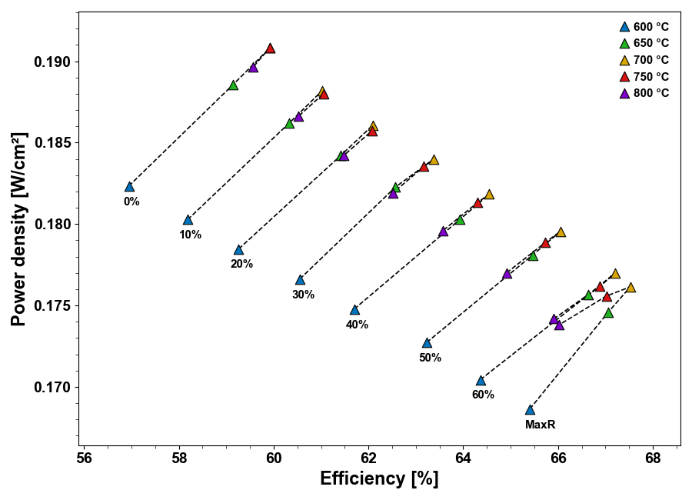
\includegraphics[width=\linewidth]{image13.png}
\caption{}
\end{subfigure}%
\hfill
\begin{subfigure}{0.49\linewidth}
\centering
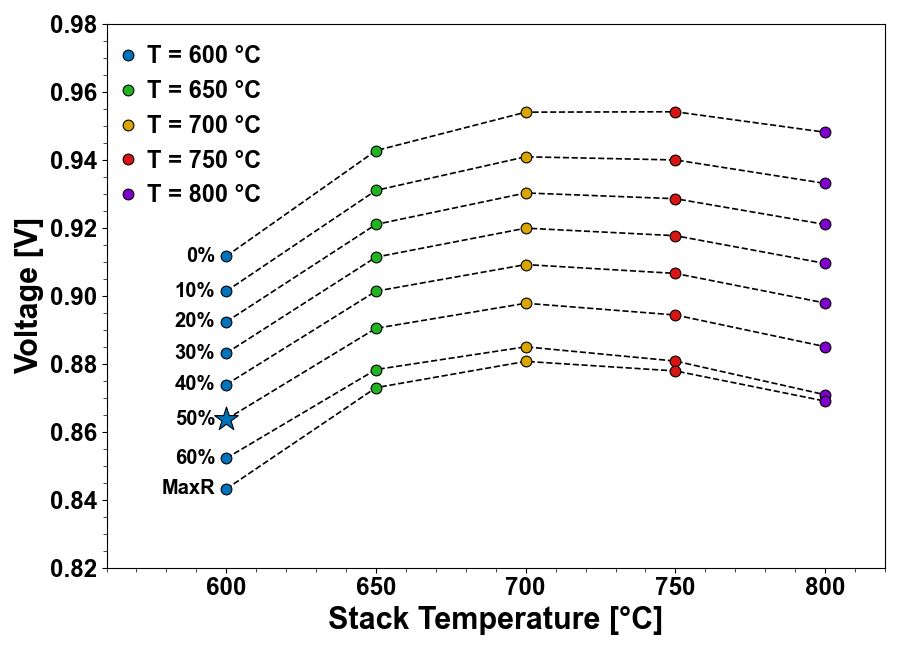
\includegraphics[width=\linewidth]{image14.png}
\caption{}
\end{subfigure}%
\caption{Performance map showing (a) efficiency and power density and (b) voltage as a function of \(T_{stack}\) and AOGR ratio.}
\label{fig:temperature-map}
\end{figure*}

The origin of this behavior can be explained by the dependence of equilibrium potential on temperature and anode gas compositions, as higher temperatures reduce the OCV through the Nernstian term of the OCV expression.
The reversible cell voltage of the SOFC is given by Eq.~\eqref{eq:nernst} where the second term on the right-hand side---the Nernstian term---is responsible for the temperature dependence of the OCV under the operating conditions of interest.
As the AOGR ratio increases, the recirculated stream depletes hydrogen partial pressure \(p_{H_{2}}\) and enriches the steam partial pressure \(p_{H_{2}O}\) at the stack anode inlet, which reduces the partial pressure ratio inside the logarithm to a value below unity and renders the logarithmic argument increasingly negative in sign.
Therefore, at higher AOGR ratios, a given temperature increment produces a larger reduction in the Nernstian term and therefore a steeper decline in the OCV.
To quantify the amplification of the OCV-reduction effect with AOGR, the magnitude of the OCV temperature sensitivity, \(\left|dOCV/dT\right|\), is shown in Supplementary Figure SX.
This finding suggests that the design and operation of NH$_3$-fueled SOFC systems incorporating AOGR should explicitly account for the coupling between the AOGR ratio and \(T_{stack}\), rather than treating the two parameters as independently optimizable variables.
In particular, when high AOGR ratios are desired for system efficiency reasons, operating the stack at moderately high temperatures yields superior overall performance compared to operating at the upper end of the temperature range.

\section{Conclusions}

A comprehensive parametric investigation of an ammonia-fueled SOFC system incorporating anode off-gas recirculation (AOGR) was conducted to clarify both the operating limits imposed on the AOGR ratio and the influence of the AOGR ratio on the overall system performance.
An integrated thermodynamic system model based on validated component models---including a 1-D SOFC stack, shell-and-tube heat exchanger, packed-bed ammonia reformer, and critical-mode ejector---was constructed, and three operating parameters (\({FU}_{stack}\), \emph{j}, and \(T_{stack}\)) were systematically varied together with the AOGR ratio.
The principal findings are summarized as follows.

\begin{itemize}
\item The maximum allowable AOGR ratio is governed by the pressure-balance constraint of the AOGR loop, in which the ejector pressure lift must overcome the cumulative pressure drops along the recirculation path.
Increasing \({FU}_{stack}\) expands this limit modestly by reducing the cracker cold-side pressure drop, whereas increasing \emph{j} narrows it substantially due to the larger anode-side flow rate and the longer cracker length required to meet the elevated heat-duty demand.
\item \(T_{stack}\) limits the maximum allowable AOGR ratio through a fundamentally distinct mechanism.
The elevated entrained flow temperature degrades the entrainment and pressure lift performance of the ejector, thereby reducing the maximum allowable AOGR ratio more sharply than what the pressure drop alone would predict.
\item Under varying \({FU}_{stack}\), the AOGR ratio induces a strongly asymmetric trade-off: the efficiency gain is highly sensitive to \({FU}_{stack}\), whereas the power density penalty remains nearly insensitive to it.
AOGR is therefore most advantageous at low \({FU}_{stack}\), where a substantial efficiency improvement is achieved at the same power density cost as at high \({FU}_{stack}\).
\item Under varying \emph{j}, the dominant trade-off shifts from the stack level to the balance-of-plant level, giving rise to a non-monotonic efficiency trajectory at high \emph{j}.
The air blower parasitic power, amplified by the elevated air flow rate and the increased BoP pressure drops, eventually overcomes the benefit of reduced fuel input.
Consequently, the optimal AOGR ratio lies below the maximum allowable value identified from the pressure-balance constraint.
\item Under varying \(T_{stack}\), the optimal operating temperature shifts downward as the AOGR ratio increases, since the AOGR-induced enrichment of steam at the anode inlet amplifies the OCV temperature sensitivity.
The resulting steeper OCV decline at higher temperatures overwhelms the modest overpotential reduction available under low-current-density operation, so that operation at the upper end of the investigated temperature range no longer yields the best performance under high AOGR conditions.
\end{itemize}

These findings demonstrate that the AOGR ratio cannot be treated as an independently optimizable variable in NH$_3$-fueled SOFC systems, since both its operating limits and its influence on system performance are tightly coupled to the underlying operating conditions through three distinct physical mechanisms: hydrodynamic resistance in the cracker, balance-of-plant parasitic power, and ejector mixing dynamics combined with OCV temperature sensitivity.
The performance maps derived in this work provide quantitative guidance for selecting the AOGR ratio in conjunction with each operating parameter and offer practical design insights for NH$_3$-fueled SOFC systems targeting marine power generation applications.

Despite the comprehensive scope of the present analysis, several limitations should be acknowledged and addressed in future work.
First, the geometrical design variables of the balance-of-plant components---including the shell-and-tube heat exchanger and the packed-bed ammonia reformer---were not individually optimized for each operating condition examined in this study, although their dimensions were resized when the heat-duty requirements could not be satisfied.
A condition-specific optimization of these geometrical variables could further refine the trade-offs identified in this work and yield more accurate quantification of the AOGR-induced parasitic power growth.
Second, the present analysis was based on a single fixed system layout---the modified Ejector CG configuration---and alternative system architectures such as blower-driven recirculation, hybrid ejector--blower configurations, or layouts with different heat integration schemes were not considered, even though such variations may shift the location of the dominant trade-off mechanism and the resulting optimal AOGR ratio.
Third, stack durability and material degradation under prolonged AOGR operation were not included in the present scope, although the AOGR-induced enrichment of steam at the anode inlet identified in this work suggests that long-term durability considerations could further constrain the practical AOGR operating window beyond the steady-state thermodynamic limits established here.
Future work should therefore extend the present framework by performing condition-specific optimization of the BoP geometries, comparatively evaluating alternative system layouts, and integrating stack durability models to translate the system-level design insights of this study into long-term operating guidelines for NH$_3$-fueled SOFC systems.

\section*{Declaration of competing interest}
The authors declare that they have no known competing financial interests or personal relationships that could have appeared to influence the work reported in this paper.

\section*{Data availability}
Data will be made available on request.

\section*{Acknowledgements}
To be completed by the authors before submission.

% Bibliography intentionally omitted at this stage.
% Uncomment and edit the following lines after preparing references.bib.
\bibliographystyle{elsarticle-num}
\bibliography{references}

\end{document}
